\section{Runtime Architecture and Asynchronous Data Path}
\label{sec:runtime}

The runtime realizes a validated plan without allowing implementation details to escape its memory proof. This requires explicit ownership of buffers, task dependencies, storage requests, kernel workspaces, and state versions.

\subsection{Core components}

The reference architecture contains the following independently testable components.

\begin{description}[style=nextline]
  \item[\code{ExecutionEngine}] Owns session lifecycle, plan validation, request admission, safe points, cancellation, and terminal status.
  \item[\code{MemoryBroker}] Owns per-tier arenas, resource credits, leases, epochs, reserves, fragmentation accounting, and high-water telemetry.
  \item[\code{VirtualTensorManager}] Resolves logical tiles to physical regions, versions, aliases, replicas, codecs, and integrity metadata.
  \item[\code{TensorStore}] Provides asynchronous bounded reads/writes, range validation, cache hints, atomic commit, and backend-specific direct paths.
  \item[\code{TransferEngine}] Moves tiles between tiers, owns copy streams/queues and events, and exposes overlap capabilities.
  \item[\code{TaskScheduler}] Maintains dependency-ready queues, atomically admits resource vectors, applies priorities and aging, and processes completions.
  \item[\code{Backend}] Provides kernels, streams/queues, events, fixed workspace algorithms, device telemetry, and deterministic capability declarations.
  \item[\code{KVManager}] Allocates logical KV pages, sharing and copy-on-write, eviction, prefetch, and request cleanup.
  \item[\code{PlanExecutor}] Instantiates operator task templates for concrete tile coordinates and binds leases to kernel arguments.
  \item[\code{Telemetry}] Emits traces, counters, structured logs, plan IDs, byte accounting, cache state, numeric diagnostics, and fault records.
\end{description}

Public APIs depend on interfaces, not concrete CUDA or Linux classes. Backend implementations may use Python for orchestration and C++, Rust, CUDA, HIP, Metal, or SYCL for critical paths, but the ownership model is uniform.

\subsection{Memory broker and arenas}

For each guaranteed tier, the broker initializes one or more arenas with size classes aligned to common tile buffers. Device arenas should be created after backend contexts and fixed library reserves so their capacity reflects those costs. Host pinned arenas are intentionally small rings; pageable cache and spill have separate quotas.

A \emph{lease} contains arena, offset, size, alignment, access mode, owner task, epoch, and terminal event. It is move-only in native code and cannot outlive its arena. Views borrow from a lease and cannot be stored in long-lived plugin state. Debug builds poison recycled buffers and validate epochs to detect use-after-release.

Fragmentation is bounded by design. Candidate tile sizes map to a finite set of size classes, and the planner charges class-rounded bytes. Large persistent allocations use dedicated segments. Coalescing allocators may be provided for irregular CPU spill, but the device guarantee must not depend on a best-effort global caching allocator.

\subsection{Atomic admission}

A task descriptor contains its complete resource vector. The scheduler calls
\[
  \operatorname{try\_lease}(\mathbf r(u))
\]
under one broker transaction. Success returns all leases; failure returns none. The task remains ready and is reconsidered when relevant credits are released. This no-partial-hold rule establishes the progress theorem and makes backpressure explicit.

Some resources are capacities rather than memory: number of asynchronous reads, copy-stream slots, compute queues, decompressor workers, file descriptors, and journal transactions. They are credits in the same vector, preventing a task from occupying memory while waiting indefinitely for an unbounded external queue.

\subsection{Task graph}

A materialized operator tile expands to typed tasks such as
\[
\begin{aligned}
\textsc{Read}&\to\textsc{Verify}\to\textsc{Decode}\to\textsc{Copy}\\
&\to\textsc{Compute}\to\textsc{Reduce}\to\textsc{Commit}\to\textsc{Evict}.
\end{aligned}
\]
Tasks are idempotent or explicitly non-idempotent. Immutable reads, verification, decode, and pure compute are retryable. A mutable commit uses a transaction ID and exactly-once version rule. The executor never repeats a non-idempotent task after an ambiguous failure without consulting the journal.

Each edge may carry an event and a virtual-tensor version rather than a host synchronization. Device compute waits on transfer events; downstream device kernels wait on compute events; host callbacks only update scheduler state after events signal. Blocking synchronization is reserved for safe points, debugging, or backends that lack asynchronous primitives.

\subsection{Asynchronous pipeline}
Figure~\ref{fig:pipeline} shows the steady-state overlap pattern used only when the selected storage and backend capabilities permit it.

\begin{figure}[H]
\centering
\resizebox{\linewidth}{!}{%
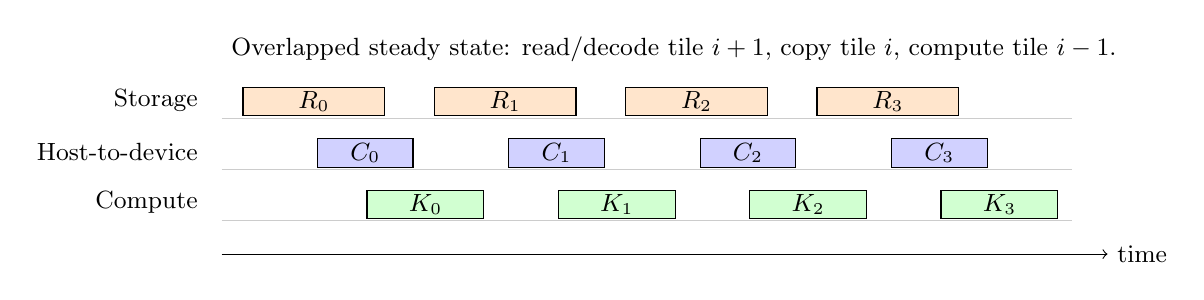
\begin{tikzpicture}[x=0.9cm,y=0.65cm,font=\small]
  \draw[->] (0,0) -- (12.5,0) node[right] {time};
  \foreach \y/\name in {3/Storage,2/Host-to-device,1/Compute}{
    \node[anchor=east] at (-0.2,\y) {\name};
    \draw[gray!40] (0,\y-0.35) -- (12,\y-0.35);
  }
  \foreach \i in {0,...,3}{
    \pgfmathsetmacro{\x}{0.3+2.7*\i}
    \draw[fill=orange!20] (\x,2.7) rectangle ++(2.0,0.55)
      node[midway] {$R_{\i}$};
    \draw[fill=blue!18] (\x+1.05,1.7) rectangle ++(1.35,0.55)
      node[midway] {$C_{\i}$};
    \draw[fill=green!18] (\x+1.75,0.7) rectangle ++(1.65,0.55)
      node[midway] {$K_{\i}$};
  }
  \node[align=left,anchor=west] at (0,4.0) {Overlapped steady state: read/decode tile $i+1$, copy tile $i$, compute tile $i-1$.};
\end{tikzpicture}%
}
\caption{Illustrative three-stage tile pipeline. Actual overlap is capability- and contention-dependent; event lifetimes retain every source and destination buffer.}
\label{fig:pipeline}
\end{figure}

On Linux, storage adapters may use \code{io\_uring}, asynchronous pread, memory mapping, or a direct-IO path. Windows and macOS use platform-native equivalents. Direct storage-to-device DMA such as GPUDirect Storage may bypass the pinned ring where supported \cite{nvidia_gds}; the portable path is storage to bounded host buffers to the device. The API exposes a task, not a specific syscall, so the planner can cost each path.

A pipeline slot is a compound lease. Slot reuse waits for the latest event touching each constituent buffer. Read cancellation does not immediately free a buffer if the OS or DMA engine can still write to it. Backends must provide a quiescence primitive used during cancellation and shutdown.

\subsection{Scheduling policy}

Ready tasks are partitioned into priority classes:

\begin{enumerate}
  \item latency-critical decode tasks on the active token frontier;
  \item tasks that unblock scarce buffers or complete a reduction;
  \item prefetch tasks on the predicted critical path;
  \item prefill and throughput batch tasks;
  \item cache population, repacking, verification, and maintenance.
\end{enumerate}

Within a class, the scheduler uses critical-path estimate, deadline slack, locality benefit, and age. Aging prevents starvation. Resource-aware selection prefers a set of tasks whose vectors fit without fragmenting size classes, but it cannot reorder a deterministic reduction beyond its declared merge tree.

A request can be assigned a weighted fair-share budget. Multi-tenant mode isolates device credits, host cache, pinned buffers, IO depth, and spill quota; it does not merely prioritize queues while allowing one tenant to occupy all memory.

\subsection{Caching and eviction}

Caches are optional performance layers above virtual storage. Entries are immutable parameter tiles, decoded packs, activation checkpoints, or clean KV pages. Cache keys include content version, logical tile, physical layout, dtype/codec, backend pack version, and numerical mode.

Eviction uses cost-aware recency:
\[
  \operatorname{value}(e)
  =\frac{p_{\mathrm{reuse}}(e)\cdot t_{\mathrm{reload}}(e)
  +t_{\mathrm{recompute}}(e)}{\bytes(e)}.
\]
This score is applied after mandatory pin and dirty-state rules. Decode-critical weights may be protected; large one-use prefill tiles are evicted quickly. The cache consumes broker credits and can be shrunk to zero without invalidating correctness.

Dirty mutable tiles follow writeback or write-through policy. Inference KV pages may be dropped if they can be rematerialized under policy, but ordinary exact mode writes them to the selected lower tier before eviction. Training parameters and optimizer state require transactional writeback.

\subsection{Storage layer}

\code{TensorStore} is a logical interface with adapters for:

\begin{itemize}
  \item read-only safetensors and sharded safetensors;
  \item memory-mapped native checkpoint ranges;
  \item the AMS packed container in Appendix~\ref{app:formats};
  \item local filesystem buffered and direct IO;
  \item optional TensorStore/Zarr-style chunked arrays \cite{tensorstore};
  \item optional direct device IO;
  \item testing stores that inject delay, short reads, corruption, and failure.
\end{itemize}

A read request specifies storage object, byte ranges, destination capability, expected checksum, priority, deadline class, and cancellation token. The adapter may coalesce adjacent ranges but must preserve the mapping to logical tiles. It validates every offset and length with overflow-safe arithmetic before issuing IO.

The checkpoint is never deserialized through executable pickle in the trusted default path. Safetensors-style metadata and explicit tensor bytes are preferred \cite{safetensors}. PyTorch checkpoints may be imported in a conversion sandbox using metadata-only and memory-mapped loading where available \cite{pytorch_serialization}.

\subsection{Backend abstraction}

A backend capability record includes:

\begin{itemize}
  \item device kind, count, topology, memory capacities, and allocation alignment;
  \item supported storage/compute dtypes and conversions;
  \item kernel catalog, shape constraints, deterministic variants, and workspace bounds;
  \item streams/queues, event semantics, asynchronous copy paths, and copy-engine counts;
  \item peer access and collective support;
  \item direct storage capability;
  \item timer resolution and profiling support;
  \item minimum scalar or vector fallback.
\end{itemize}

The core implementation should support a CPU backend first because it is the universal semantic reference. CUDA, ROCm/HIP, Metal/MPS, XPU/SYCL, Vulkan, or other backends are plugins. ``Hardware agnostic'' means that the graph and virtual tensor contracts are portable and every supported backend has a safe fallback; it does not mean that one kernel binary or identical tile shape is optimal everywhere.

\subsection{Fault handling and recovery}

Every terminal error propagates through dependent tasks, which are cancelled before admission. Already submitted tasks are quiesced; their leases remain valid until events finish. Immutable corrupted reads are retried from another replica when available. Repeated checksum mismatch marks the storage object unhealthy and terminates with evidence.

Mutable commits use:

\begin{enumerate}
  \item write new tile bytes to a temporary region;
  \item flush according to durability policy;
  \item record checksum and target logical version in a write-ahead journal;
  \item atomically publish the region map update;
  \item retire the old version after readers release it;
  \item truncate or checkpoint the journal.
\end{enumerate}

Inference without durable sessions can choose a lighter policy. Training checkpoints must use a crash-consistent policy and record RNG, optimizer, scaler, and scheduler state.

\subsection{Observability}

Every request trace records plan ID and, subject to cardinality controls:

\begin{itemize}
  \item current and peak leases by tier, class, and owner;
  \item logical and physical bytes read/written by path;
  \item read-size histogram, queue depth, bandwidth, and latency;
  \item host/device copy overlap and idle gaps;
  \item kernel time, workspace, tile shapes, and achieved arithmetic rate;
  \item cache hits, evictions, prefetch usefulness, and recomputations;
  \item scheduler ready/wait times and resource-blocking reasons;
  \item KV page residency and spill;
  \item numerical diagnostics and deterministic-mode identifiers;
  \item retries, integrity failures, replans, cancellations, and cleanup time.
\end{itemize}

Metrics expose OpenTelemetry/Prometheus-compatible instruments, while a binary trace preserves high-rate task events. Tensor contents are not logged by default. A plan simulator consumes traces to compare predicted and actual stage costs.
